\documentclass[tikz]{standalone}
\usetikzlibrary{positioning}

\begin{document}
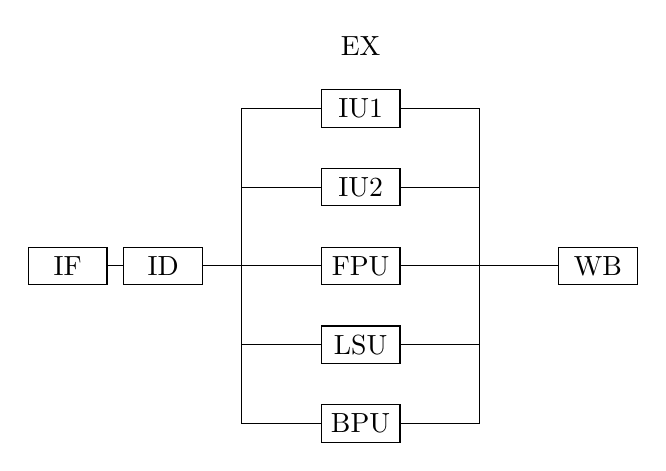
\begin{tikzpicture}[every node/.style={draw, minimum width=1cm}]
    \node(if) at (0, 0) {IF};
    \node[right=2mm of if](id) {ID};
    \draw (id) -- ++(1, 0) coordinate(midway);
    \draw (midway)
    -- ++(0, 2)
    -- ++(1, 0) node[anchor=west](iu1) {IU1}
    (iu1.north) ++(0, 0.3) node[draw=none, anchor=south]{EX};

    \draw (if.east)--(id.west)
    (iu1.east) -- ++(1, 0) -- ++(0, -2) -- ++(1, 0)
    node[anchor=west](wb){WB};

    \draw (midway) ++(0, 1)
    -- ++(1, 0) node[anchor=west] (iu2){IU2}
    (iu2.east) -- ++(1, 0);
    \draw (midway) -- ++(1, 0)
    node[anchor=west] (fpu){FPU}
    (fpu.east) -- ++(1, 0);
    \draw (midway)
    -- ++(0, -2)
    -- ++(1, 0) node[anchor=west] (bpu) {BPU}
    (bpu.east) -- ++ (1, 0)
    -- ++(0, 2)
    ;

    \draw (midway) ++(0, -1)
    -- ++(1, 0)
    node[anchor=west](lsu) {LSU}
    (lsu.east) -- ++(1, 0)
    ;
\end{tikzpicture}
\end{document}
